\chapter{Nacimiento del proyecto}\label{nacimiento}

Uno de los mayores intereses del autor de este proyecto en el mundo del software siempre ha sido el uso de técnicas de inteligencia artificial para resolver problemas actuales.

Aprovechando que cursaba la asignatura de Procesamiento de Imágenes Digitales con la profesora María José Jiménez Rodríguez para preguntarle si sabía de algún TFG en el que estuviesen involucradas imágenes y pudiese desarrollar una solución de inteligencia artificial. La principal motivación par esto era que nunca había trabajado con imágenes digitales en el ámbito de machine learning.

María José habló sobre un proyecto muy interesante dirigido por el investigador Luis María Escudero Cuadrado del Departamento de Biología Celular de la Universidad de Sevilla. Parte de este este proyecto consistía en procesar imágenes 3D de glándulas salivales tomadas por un microscopio confocal para obtener la segmentación de las células. Un punto importante era que este procesado fuese automático ya que se podría ahorrar mucho tiempo, por lo que estaban valorando el uso de técnicas de machine learning.

Tras ver que este proyecto era interesante se planeó una primera visita al Departamento de Biología Celular, siendo recibidos por Luis María Escudero, Pablo Vicente-Manuera y Pedro Gómez-Gálvez. En esta reunión se habló en más detalle sobre la investigación que realizaban y el problema que se iba a abordar en el TFG.

Estaban estudiando la arquitectura a nivel celular del tejido epitelial. El tejido epitelial es uno de los 4 tejidos animales básicos, por lo que gran parte del organismo está compuesto por éste. Aunque las células de este tejido siempre se han representado en forma de prisma (cuando las células están en el mismo plano) o en forma de tronco (cuando se produce un pliegue), han demostrado que en condiciones de curvatura adoptan forma de escutoide para estabilizar energéticamente el tejido. La forma geométrica escutoide fue descubierta por este grupo de investigación \cite{GomezGalvez2018}. En la figura \ref{fig:tejidoepitelial} se pueden ver las forma de prisma, tronco y escutoide.

\figura{1}{img/tejidoepitelial}{\textbf{a} Representación de las células del tejido epitelial cuando están en una estructura plana. Se suele representar en forma de prisma. \textbf{b} Representación de las células del tejido epitelial cuando se produce un pliegue. Se suele representar en forma de tronco. \textbf{c} Geometría propuesta caracterizada por tener al menos un vértice en un plano distinto al de sus dos bases. En la figura de arriba se ven dos elementos adyacentes con forma escutoide. En la figura de abajo se ven estos elementos por separado. Las células del tejido epitelial tendrían esta geometría. (Figura editada procedente de Gómez-Gálvez et. al 2018)}{fig:tejidoepitelial}{}{Formas geométricas prisma, tronco y escutoide}

Para obtener un modelo visual del tejido epitelial empiezan utilizando un microscopio confocal del que obtienen un stack de imágenes 2D, consiguiendo así una imagen 3D. Esta imagen es procesada computacionalmente utilizando herramientas de MATLAB y Fiji (ImageJ) para conseguir una imagen con todas las células etiquetadas correctamente, proceso conocido como segmentación semántica. El resultado final sería una imagen en la que cada vóxel del fondo tiene valor 0 y los vóxeles pertenecientes a cada célula tienen valor $1,2,3...n$, donde $n$ es el nº de células en la imagen. Un ejemplo de dos capas de la imagen 3D original y la imagen etiquetada puede verse en la figura \ref{fig:ejemplo1_segmentacion}

\begin{figure}[ht]
\centering
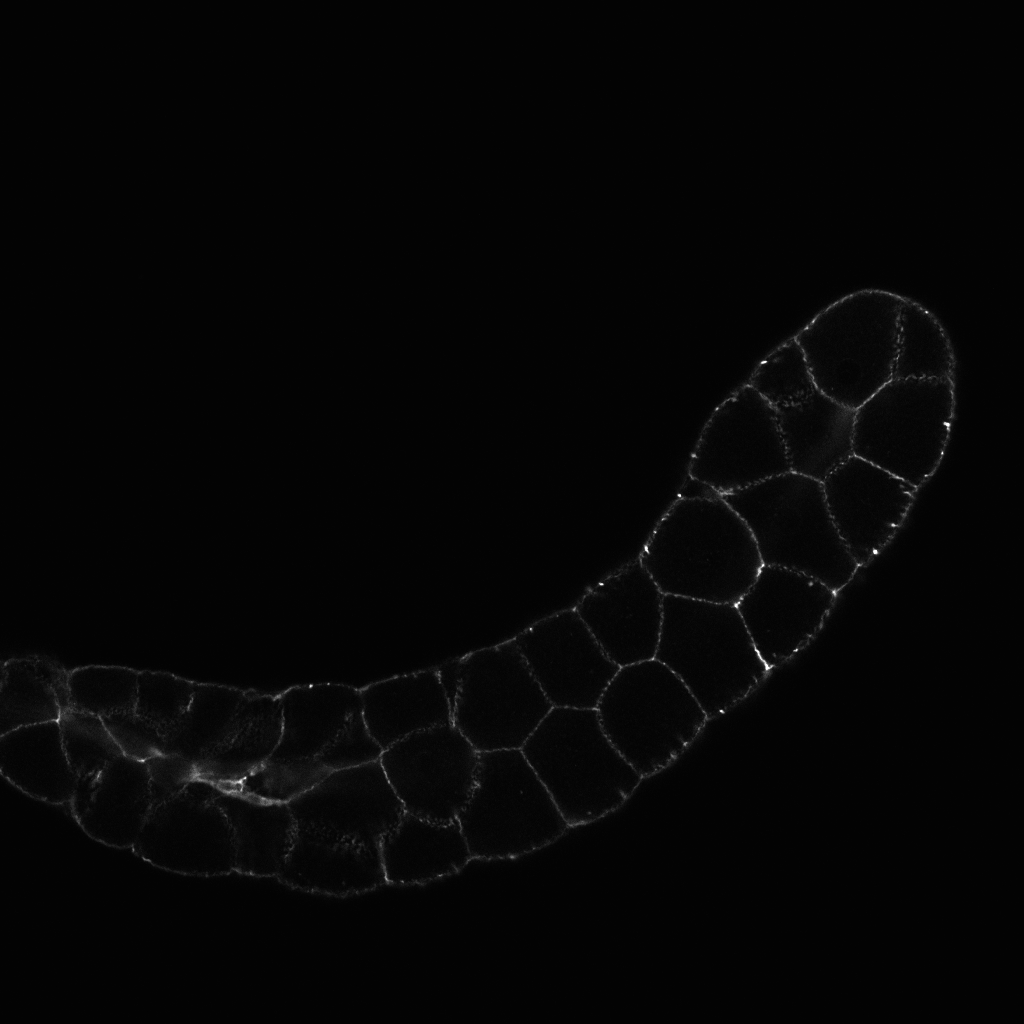
\includegraphics[scale=0.18]{img/raw 04_1a Z=77.png}
\vspace*{1mm}
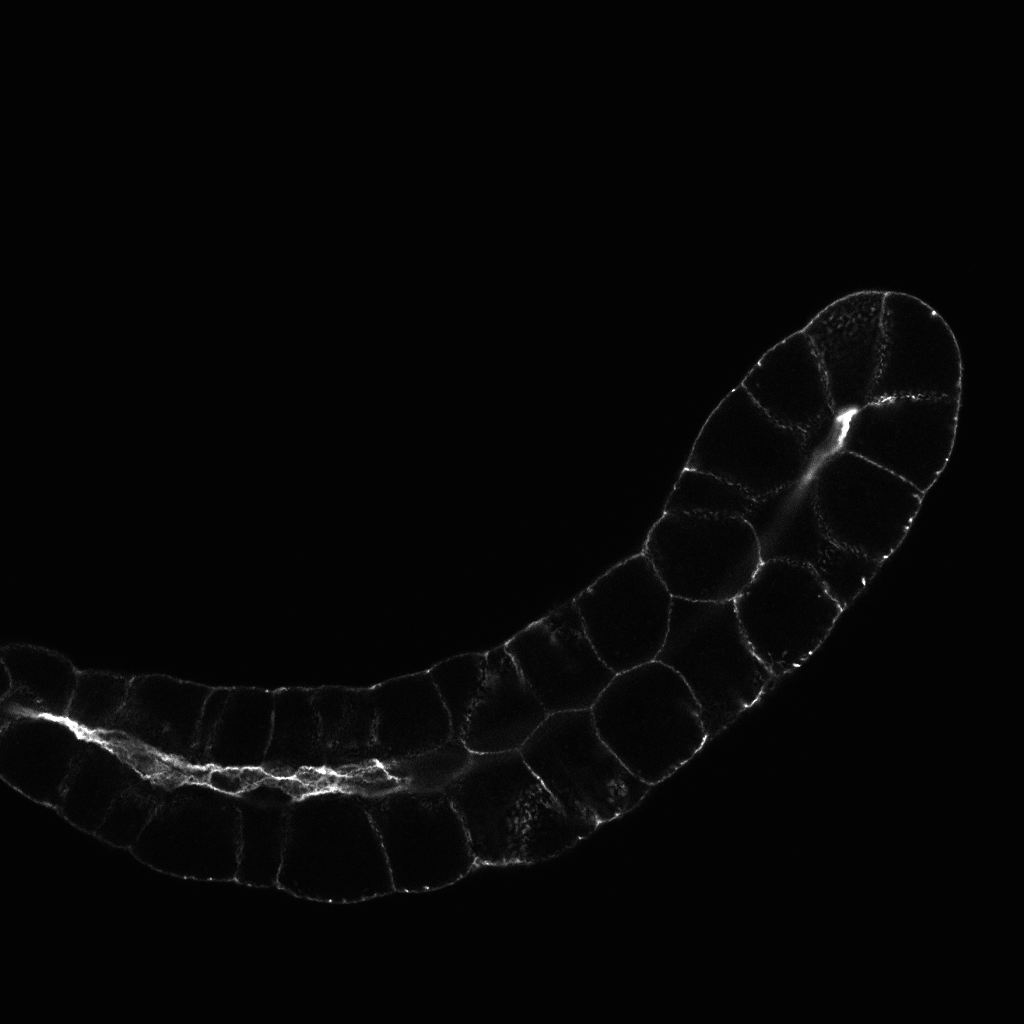
\includegraphics[scale=0.18]{img/raw 04_1a Z=100.png}
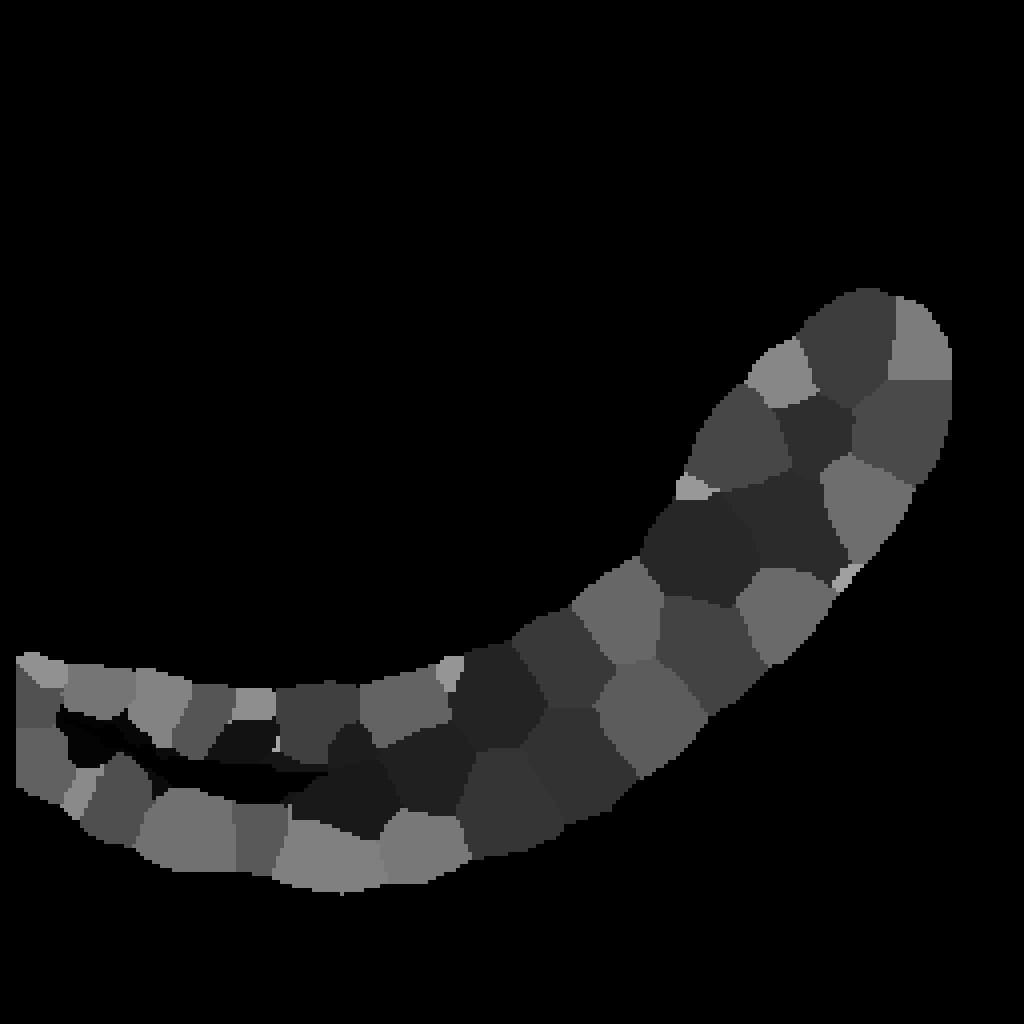
\includegraphics[scale=0.18]{img/target 04_1a Z=77.png}
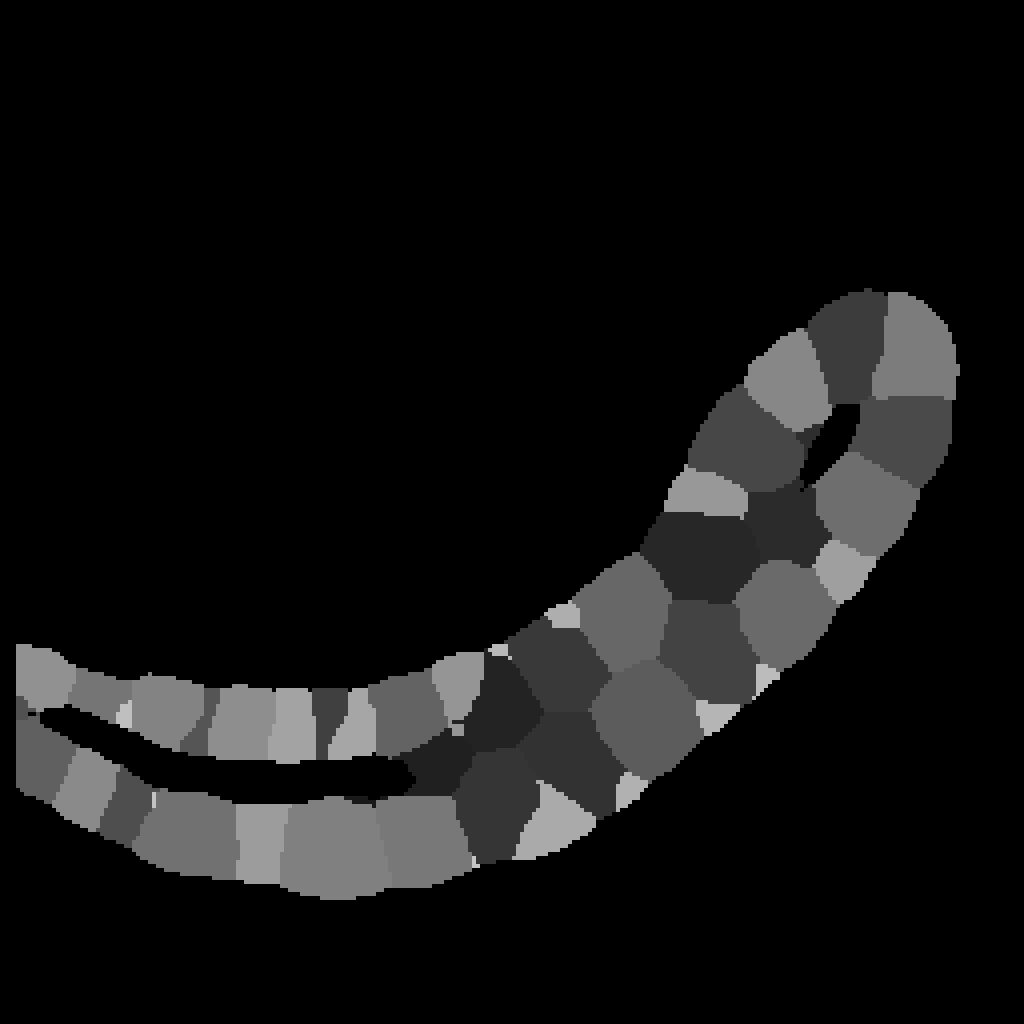
\includegraphics[scale=0.18]{img/target 04_1a Z=100.png}
\caption[Segmentación de dos capas de una glándula salivar de Drosophila]{Esta figura muestra el resultado de aplicar el procesado a la imagen 3D de una glándula salivar de Drosophila (un género de moscas), obtenida por microscopía. La imagen tiene las dimensiones $1024*1024*234$, seleccionándose para su representación Z=77 y Z=100. En la primera fila se muestra la imagen obtenida por microscopía y la segunda fila se muestra la obtenida al aplicar segmentación a las células. En la primera columna se muestra la capa Z=77 y en la segunda la capa Z=100.}\bigskip
\label{fig:ejemplo1_segmentacion}
\end{figure}

Pasar de la primera fila de la figura \ref{fig:ejemplo1_segmentacion} a la segunda fila es un proceso que puede llevar hasta una semana ya que se quiere conseguir un etiquetado perfecto. Esto provoca que se invierta mucho tiempo en una tarea repetitiva y poco interesante y se reste tiempo de las tareas de interés científico. Querían reducir el tiempo necesario para la segmentación y para ello pensaron que sería buena idea recurrir a técnicas de machine learning. Sería el objetivo principal del TFG, por tanto, obtener una segmentación automática que redujera el tiempo de segmentación manual, siendo lo ideal obtener directamente la segmentación perfecta.